\documentclass[a4j,12pt]{jarticle}
\bibliographystyle{junsrt}
\usepackage{amsmath}
\usepackage{amssymb}
%\usepackage{listing}
\usepackage[dvipdfmx]{graphicx}
\usepackage{url}
\usepackage{color}
\usepackage{listings}
\usepackage{latexsym}

\def\theequation{\thesection.\arabic{equation}}
\makeatletter
\@addtoreset{equation}{section}
\makeatother

\makeatletter
 \renewcommand{\thefigure}{%
   \thesection.\arabic{figure}}
  \@addtoreset{figure}{section}
\makeatother

\setlength{\topmargin}{20mm}
\addtolength{\topmargin}{-1in}
\setlength{\oddsidemargin}{20mm}
\addtolength{\oddsidemargin}{-1in}
\setlength{\evensidemargin}{15mm}
\addtolength{\evensidemargin}{-1in}
\setlength{\textwidth}{170mm}
\setlength{\textheight}{254mm}
\setlength{\headsep}{0mm}
\setlength{\headheight}{0mm}
\setlength{\topskip}{0mm}
\def\vector#1{\mbox{\boldmath $#1$}}
\lstdefinestyle{myCustomMatlabStyle}{
  language=C++,
  tabsize=3,
  showspaces=false,
  showstringspaces=false,
  frame=tb,
  keywordstyle={\color{red}},
  keywordstyle={[2]\color{green}},
  keywordstyle={[3]\color{pink}},
  emph={void,const,int,vector},
  emphstyle={\color{blue}},
  captionpos=b
}
\renewcommand{\refname}{文献リスト}

\title{周期境界条件について}
\author{糸賀 響}
\date{\today}

\begin{document}
\maketitle \thispagestyle{empty}
\section{周期境界条件PBCとは}
単位セルを連続すると考えることで、有限大きさの1つセル(基本セル)の中にのみに粒子や計算対象の物体を実体化させるにも関わらず、
無限サイズの系を模倣することができる条件(モデル)のことを周期境界条件という(イメージ図\ref{fig:pbc})。
3 次元の場合、最も簡単なものは一辺の長さが $L$ の立方体を基本セルとし、そのまわりに同じサイズをもち基本セルの内容の虚像をもつイメージセルを考えるものだろう。
\begin{figure}[htbp]
   \begin{center}
   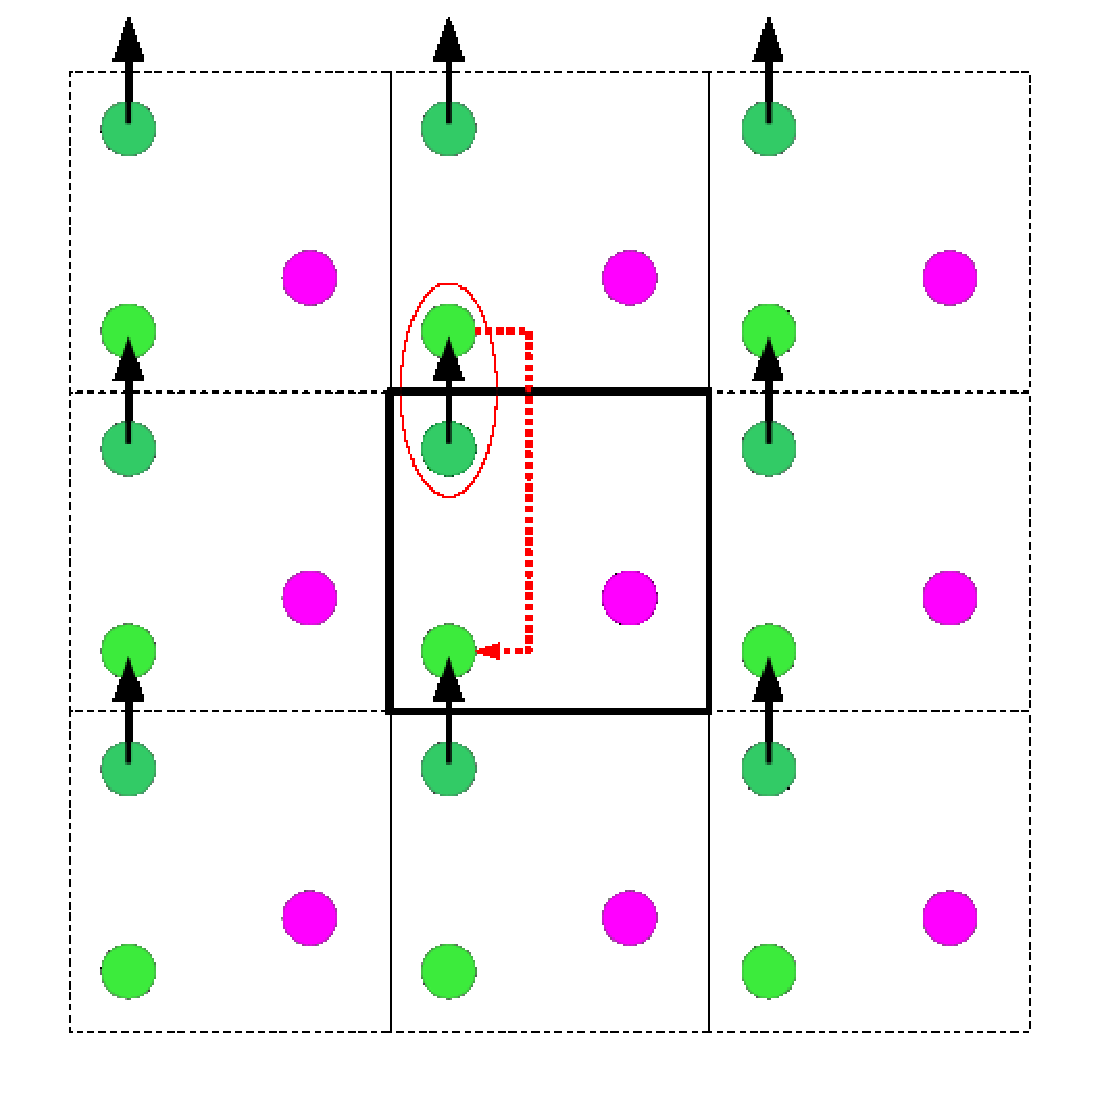
\includegraphics[,width=0.5\textwidth]{fig/pbc.eps}
   \end{center}
   \caption{
   \label{fig:pbc}
      周期境界条件のイメージ図
   }
\end{figure}

任意次元の周期境界では、$i$ 番目の粒子を
\begin{eqnarray}
   \vector{p}_i = \vector{p}_i+\vector{L_1} = \vector{p}_i+\vector{L_2} = \ldots
\end{eqnarray}
のように粒子の位置を考える。
$\{\vector{L}\}$ は線型独立なベクトルであり、それぞれ$L$ の整数倍のスカラーを要素にもつ。

\end{document}

